% !TEX program = LuaLaTeX
%\errorcontextlines 10000
\DocumentMetadata{lang=en,testphase=latest,uncompress,
  pdfversion=1.7,pdfstandard=ua-1,
%  pdfversion=2.0,pdfstandard=ua-2,
%  pdfstandard=a-4f,
}
\documentclass{article}

\usepackage{tikz}
\newcommand{\fp}{f'}
\newcommand{\fpp}{f''}
\newcommand{\tbox}[1]{\tagpdfsetup{table/tagging=presentation}\begin{tabular}{c}#1\end{tabular}} % a tall box
\title{Title}

\begin{document}

%\noindent before\\
%\begin{tikzpicture}
%  \matrix {
%    & \node (A) {A}; \\
%    \node{B};&& \node(C){C}; \\
%  };
%  \draw (A.south) -- (A|- C.south);
%\end{tikzpicture}\\
%after
%\end{document}

concline1Src.tex

\begin{tikzpicture}[alt={f'' is negative when x<0 and positive when x>0, so that f is concave down when x<0 and concave up when x>0, and x=0 is an inflection point.}]
  \matrix[row sep=1mm,column sep=3mm,ampersand replacement=\&] {
    \&\&\& \node (tp1) {$0$}; \\[-1ex]
    \node(linestart) {$x$}; \&\&\&\&\& \node(lineend) {}; \\[-1ex]
    \&\node (fppstart) {$\fpp$}; \& \node{$-$}; \&\& \node{$+$}; \\
    \&\node (fstart) {$f$}; \& \node{CD}; \& \node{IP}; \& \node{CU}; \\
  };
  \draw [<->] (linestart.east) -- (lineend);
  \draw (fppstart.south west) -- (lineend.west |- fppstart.south);
  \draw (fppstart.east |- lineend) -- (fppstart.east|-fstart.south);
  \foreach \x in {1} {
    \draw (tp\x|-linestart)+(0,5pt) -- (tp\x |- fppstart.south);
  }
\end{tikzpicture}

concline2Src.tex

\begin{tikzpicture}[alt={f'' is negative and f is concave down when x<-1 or 0<x<1.  f'' is positive and f is concave up when -1<x<0 or 1<x.  f is not defined at ±1, and has an inflection point at 0.}]
  \matrix[row sep=1mm,column sep=3mm,ampersand replacement=\&] {
    \&\&\& \node (tp1) {$-1$}; \&\& \node (tp2) {$0$}; \&\& \node (tp3) {$1$}; \\[-1ex]
    \node(linestart) {$x$}; \&\&\&\&\&\&\&\&\& \node(lineend) {}; \\[-1ex]
    \&\node (fppstart) {$\fpp$}; \& \node {$-$}; \&\& \node {$+$}; \&\& \node {$-$}; \&\& \node {$+$}; \\
    \&\node (fstart) {$f$}; \& \node {CD}; \& \node {U}; \& \node {CU}; \& \node {IP}; \& \node {CD}; \& \node {U}; \& \node {CU}; \\
  };
  \draw [<->] (linestart.east) -- (lineend);
  \draw (fppstart.south west) -- (lineend.west |- fppstart.south);
  \draw (fppstart.east |- lineend) -- (fppstart.east|-fstart.south);
  \foreach \x in {1,2,3} {
    \draw (tp\x |- linestart)+(0,5pt) -- (tp\x |- fppstart.south);
  }
\end{tikzpicture}

concline3Src.tex

\begin{tikzpicture}[alt={f'' is negative and f is concave down when 0<t<2/√3≈1.2.  f'' is positive and f is concave up when 2/√3<t.  f has an inflection point at 2/√3.}]
  \matrix[row sep=1mm,column sep=3mm,ampersand replacement=\&] {
    \& \node (tp1) {$0$}; \&\& \node (tp2) {$\frac2{\sqrt3}\approx1.2$}; \\[-1ex]
    \node {$t$}; \& \node(linestart) {}; \&\&\&\& \node(lineend) {}; \\[-.5ex]
    \node (fppstart) {$\fpp$}; \&\& \node {$-$}; \&\& \node {$+$}; \\
    \node (fstart) {$f$}; \&\& \node {CD}; \& \node {IP}; \& \node {CU}; \\
  };
  \draw [->] (tp1 |- linestart) -- (lineend); % number line
  \draw (fppstart.south west) -- (lineend.west |- fppstart.south west); % long horiz
  \draw (tp1.south |- tp2.south) -- (tp1.south |- fstart.south); % left vert
  \foreach \x in {2} {
    \draw (tp\x.south) -- (tp\x |- fppstart.south);
  }
\end{tikzpicture}

incrdecr1fullSrc.tex

\begin{tikzpicture}
  \matrix[row sep=1mm,column sep=3mm,ampersand replacement=\&] {
    \&\&\& \node (tp1) {$-1$}; \&\& \node (tp2) {$\frac13$}; \\[-1ex]
    \node(linestart) {$x$}; \&\&\&\&\&\&\& \node(lineend) {}; \\[-1ex]
    \&\node (fpstart) {$\fp$}; \& \node {$+$}; \&\& \node {$-$}; \&\& \node {$+$}; \\
    \&\node (fstart) {$f$}; \& \node {incr}; \&\& \node {decr}; \&\& \node {incr}; \\
  };
  \draw [<->] (linestart.east) -- (lineend);
  \draw (fpstart.south west) -- (lineend.west |- fpstart.south);
  \draw (fpstart.east |- lineend) -- (fpstart.east|-fstart.south);
  \foreach \x in {1,2} {
    \draw (tp\x|-linestart)+(0,5pt) -- (tp\x |- fpstart.south);
  };
\end{tikzpicture}

incrdecr1Src.tex

\begin{tikzpicture}
  \matrix[row sep=1mm,column sep=8mm,ampersand replacement=\&] {
    \&\&\& \node (tp1) {$-1$}; \&\& \node (tp2) {$\frac13$}; \\[-1ex]
    \node(linestart) {$x$}; \&\&\&\&\&\&\& \node(lineend) {}; \\[-1ex]
    \&\node (fpstart) {$\fp$}; \\
    \&\node (fstart) {$f$}; \\
  };
  \draw [<->] (linestart.east) -- (lineend);
  \draw (fpstart.south west) -- (lineend.west |- fpstart.south);
  \draw (fpstart.east |- lineend) -- (fpstart.east|-fstart.south);
  \foreach \x in {1,2} {
    \draw (tp\x|-linestart)+(0,5pt) -- (tp\x |- fpstart.south);
  }
\end{tikzpicture}

incrdecr2Src.tex

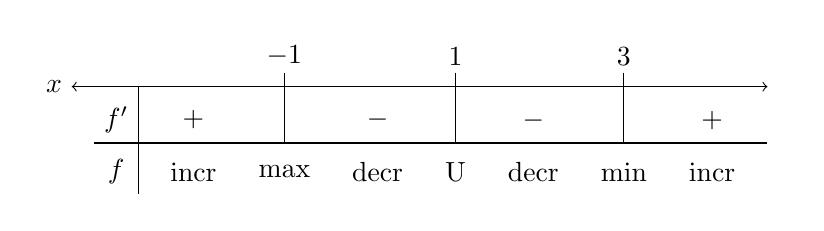
\begin{tikzpicture}
  \matrix[row sep=1mm,column sep=3mm,ampersand replacement=\&] {
    \&\&\& \node(tp1){$-1$}; \&\& \node(tp2){$1$}; \&\& \node(tp3){$3$}; \\[-1ex]
    \node(linestart){$x$}; \&\&\&\&\&\&\&\&\& \node(lineend) {}; \\[-1ex]
    \&\node(fpstart){$\fp$}; \& \node{$+$}; \&\& \node{$-$}; \&\& \node{$-$}; \&\& \node{$+$}; \\
    \&\node(fstart){$f$}; \& \node{incr}; \& \node{max}; \& \node{decr}; \& \node{U}; \& \node{decr}; \& \node{min}; \& \node{incr}; \\
  };
  \draw [<->] (linestart.east) -- (lineend);
  \draw (fpstart.south west) -- (lineend.west |- fpstart.south);
  \draw (fpstart.east |- lineend) -- (fpstart.east|-fstart.south);
  \foreach \x in {1,2,3} {
    \draw (tp\x|-linestart)+(0,5pt) -- (tp\x |- fpstart.south);
  };
\end{tikzpicture}

incrdecr3Src.tex

\begin{tikzpicture}[alt={f' is negative and f is decreasing when x<-1 or 0<x<1.  f' is positive and f is increasing when -1<x<0 or 1<x.  This means that f has a local min at x=±1 and a local max at x=0.}]
  \matrix[row sep=1mm,column sep=3mm,ampersand replacement=\&] {
    \&\&\& \node(tp1){$-1$}; \&\& \node(tp2){$0$}; \&\& \node(tp3){$1$}; \\[-1ex]
    \node(linestart){$x$}; \&\&\&\&\&\&\&\&\& \node(lineend) {}; \\[-1ex]
    \&\node(fpstart){$\fp$}; \& \node{$-$}; \&\& \node{$+$}; \&\& \node{$-$}; \&\& \node{$+$}; \\
    \&\node(fstart){$f$}; \& \node{decr}; \& \node{min}; \& \node{incr}; \& \node{max}; \& \node{decr}; \& \node{min}; \& \node{incr}; \\
  };
  \draw [<->] (linestart.east) -- (lineend);
  \draw (fpstart.south west) -- (lineend.west |- fpstart.south);
  \draw (fpstart.east |- lineend) -- (fpstart.east|-fstart.south);
  \foreach \x in {1,2,3} {
    \draw (tp\x|-linestart)+(0,5pt) -- (tp\x |- fpstart.south);
  }
\end{tikzpicture}

incrdecrTrigSrc.tex

\begin{tikzpicture}[alt={f' is positive and f is increasing when 0<x<π/3 or π<x<5π/3.  f' is negative and f is decreasing when π/3<x<π or 5π/3<x<2π.  This means that f has a local max at x=π/3 and 5π/3 and a local min at x=π.}]
  \matrix[row sep=1mm,column sep=2mm,ampersand replacement=\&] {
    \& \node(tp1){$0$}; \&\& \node(tp2){$\frac\pi3$}; \&\& \node(tp3){$\pi$}; \&\& \node(tp4){$\frac{5\pi}3$}; \&\& \node(tp5){$2\pi$}; \\[-1ex]
    \node {$x$}; \& \node(linestart){}; \&\&\&\&\&\&\&\&\& \node(lineend) {}; \\[-1ex]
    \node(fpstart){$\fp$}; \&\& \node{$+$}; \&\& \node{$-$}; \&\& \node{$+$}; \&\& \node{$-$}; \\
    \node(fstart){$f$}; \&\& \node{incr}; \& \node{max}; \& \node{decr}; \& \node{min}; \& \node{incr}; \& \node{max}; \& \node{decr};\\
  };
  \draw (tp1 |- linestart) -- (tp5 |- lineend);
  \draw (fpstart.south west) -- (tp5 |- fpstart.south);
  \draw (tp1|-linestart)+(0,5pt) -- (tp1 |- fstart.south);
  \foreach \x in {1,2,3,4,5} {
    \draw (tp\x|-linestart)+(0,5pt) -- (tp\x |- fpstart.south);
  }
\end{tikzpicture}


paramcalcSrc.tex

\begin{tikzpicture}[alt={f'' is positive and f is concave up when x<3/5.  f'' is negative and f is concave down when 3/5<x.}]
  \matrix[row sep=1mm,column sep=3mm,ampersand replacement=\&] {
    \&\&\& \node (tp1) {$\frac35$}; \\[-1ex]
    \node(linestart) {$x$}; \&\&\&\&\& \node(lineend) {}; \\[-1ex]
    \&\node (fppstart) {$\fpp$}; \& \node {$+$}; \&\& \node {$-$}; \\
    \&\node (fstart) {$f$}; \& \node {CU}; \&\& \node {CD}; \\
  };
  \draw [<->] (linestart.east) -- (lineend);
  \draw (fppstart.south west) -- (lineend.west |- fppstart.south);
  \draw (fppstart.east |- lineend) -- (fppstart.east|-fstart.south);
  \draw (tp1|-linestart)+(0,5pt) -- (tp1 |- fppstart.south);
\end{tikzpicture}

prereqMatrixSrc.tex

\begin{tikzpicture}[alt={x^2-4 is positive when x<-2 or 2<x.  x^2-4 is negative when -2<x<2.}]
  \matrix[row sep=1mm,column sep=3mm,ampersand replacement=\&]{
    \&\&\& \node (tp1) {$-2$}; \&\& \node (tp2) {$2$}; \\[-1ex]
    \node(linestart) {$x$}; \&\&\&\&\&\&\& \node(lineend) {}; \\[-1ex]
    \&\node (fstart) {$x^2-4$}; \& \node {$+$}; \&\& \node {$-$}; \&\& \node {$+$}; \\
  };
  \draw [<->] (linestart.east) -- (lineend);
  \draw (fstart.south west) -- (lineend.west |- fstart.south);
  \draw (fstart.east |- lineend) -- (fstart.east|-fstart.south);
  \foreach \x in {1,2} {
    \draw (tp\x|-linestart)+(0,5pt) -- (tp\x |- fstart.south);
  }
\end{tikzpicture}

sketch1Src.tex

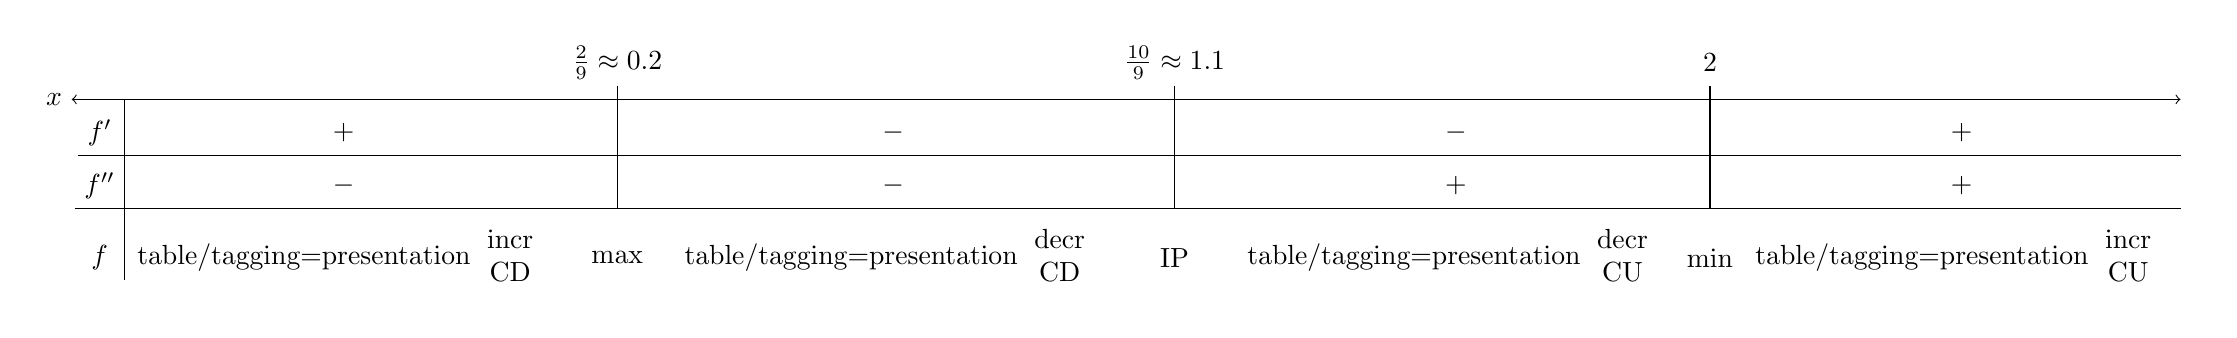
\begin{tikzpicture}
  \matrix[row sep=1mm,column sep=0.5mm,ampersand replacement=\&] {
    \&\&\& \node (tp1) {$\frac29\approx0.2$}; \&\& \node (tp2) {$\frac{10}9\approx1.1$}; \&\& \node (tp3) {$2$}; \\[-1ex]
    \node(linestart) {$x$}; \&\&\&\&\&\&\&\&\& \node(lineend) {}; \\[-1ex]
    \&\node (fpstart) {$\fp$}; \& \node {$+$}; \&\& \node {$-$}; \&\& \node {$-$}; \&\& \node {$+$}; \\
    \&\node (fppstart) {$\fpp$}; \& \node {$-$}; \&\& \node {$-$}; \&\& \node {$+$}; \&\& \node {$+$}; \\
    \&\node (fstart) {$f$}; \& \node {\tbox{incr\\CD}}; \& \node {max}; \& \node {\tbox{decr\\CD}}; \& \node {IP}; \& \node {\tbox{decr\\CU}}; \& \node {min}; \& \node {\tbox{incr\\CU}}; \\
  };
  \draw [<->] (linestart.east) -- (lineend);
  \draw (fpstart.south west) -- (lineend.west |- fpstart.south);
  \draw (fppstart.south west) -- (lineend.west |- fppstart.south);
  \draw (fppstart.east |- lineend) -- (fppstart.east|-fstart.south);
  \foreach \x in {1,2,3} {
    \draw (tp\x |- linestart)+(0,5pt) -- (tp\x |- fppstart.south);
  };
\end{tikzpicture}

sketch2Src.tex

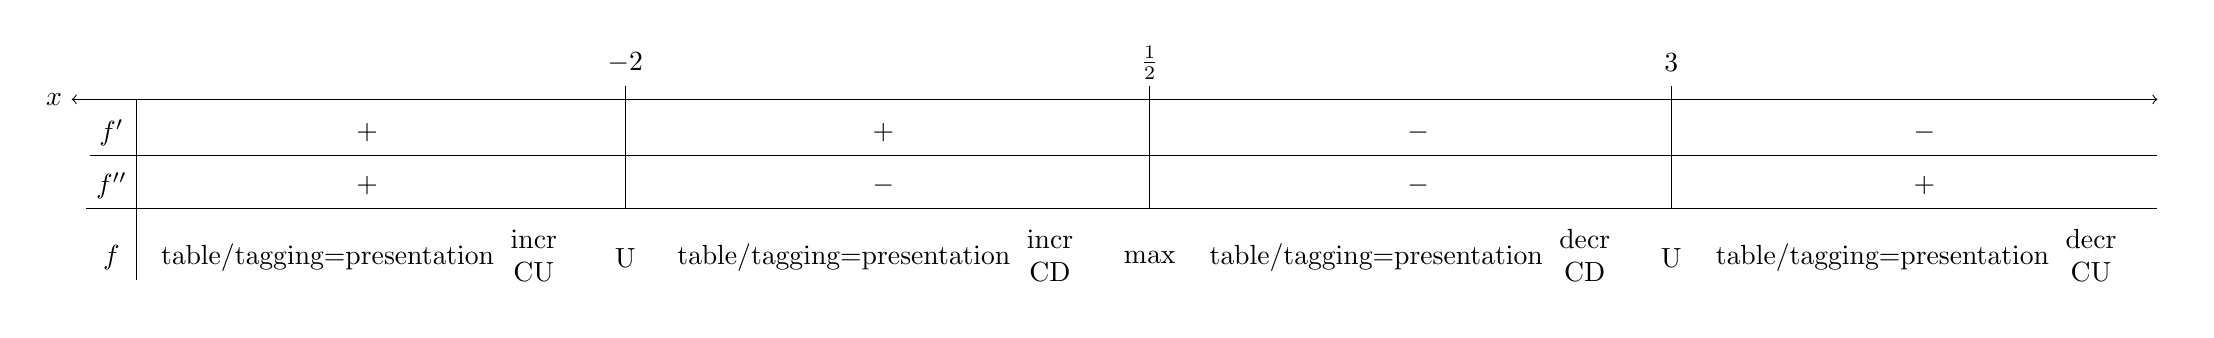
\begin{tikzpicture}
  \matrix[row sep=1mm,column sep=2mm,ampersand replacement=\&] {
    \&\&\& \node (tp1) {$-2$}; \&\& \node (tp2) {$\frac12$}; \&\& \node (tp3) {$3$}; \\[-1ex]
    \node(linestart) {$x$}; \&\&\&\&\&\&\&\&\& \node(lineend) {}; \\[-1ex]
    \&\node (fpstart) {$\fp$}; \& \node {$+$}; \&\& \node {$+$}; \&\& \node {$-$}; \&\& \node {$-$}; \\
    \&\node (fppstart) {$\fpp$}; \& \node {$+$}; \&\& \node {$-$}; \&\& \node {$-$}; \&\& \node {$+$}; \\
    \&\node (fstart) {$f$}; \& \node {\tbox{incr\\CU}}; \& \node {U}; \& \node {\tbox{incr\\CD}}; \& \node {max}; \& \node {\tbox{decr\\CD}}; \& \node {U}; \& \node {\tbox{decr\\CU}}; \\
  };
  \draw [<->] (linestart.east) -- (lineend);
  \draw (fpstart.south west) -- (lineend.west |- fpstart.south);
  \draw (fppstart.south west) -- (lineend.west |- fppstart.south);
  \draw (fppstart.east |- lineend) -- (fppstart.east|-fstart.south);
  \foreach \x in {1,2,3} {
    \draw (tp\x |- linestart)+(0,5pt) -- (tp\x |- fppstart.south);
  };
\end{tikzpicture}

sketch3Src.tex

\scriptsize
\begin{tikzpicture}
  \matrix[row sep=1mm,column sep=0mm,ampersand replacement=\&] {
    \&\&\& \node (tp1) {$-5.8$}; \&\& \node (tp2) {$-4$}; \&\& \node (tp3) {$-1.3$}; \&\& \node (tp4) {$0$}; \&\& \node (tp5) {$1.1$}; \\[-1ex]
    \node(linestart) {$x$}; \&\&\&\&\&\&\&\&\&\&\&\&\& \node(lineend) {}; \\[-1ex]
    \&\node (fpstart) {$\fp$}; \& \node {$+$}; \&\& \node {$+$}; \&\& \node {$-$}; \&\& \node {$-$}; \&\& \node {$+$}; \&\& \node {$+$}; \\
    \&\node (fppstart) {$\fpp$}; \& \node {$+$}; \&\& \node {$-$}; \&\& \node {$-$}; \&\& \node {$+$}; \&\& \node {$+$}; \&\& \node {$-$}; \\
    \&\node (fstart) {$f$}; \& \node {\tbox{incr\\CU}}; \& \node {IP}; \& \node {\tbox{incr\\CD}}; \& \node {max}; \& \node {\tbox{decr\\CD}}; \& \node {IP}; \& \node {\tbox{decr\\CU}}; \& \node {min}; \& \node {\tbox{incr\\CU}}; \& \node {IP}; \& \node {\tbox{incr\\CD}}; \\
  };
  \draw [<->] (linestart.east) -- (lineend);
  \draw (fpstart.south west) -- (lineend.west |- fpstart.south);
  \draw (fppstart.south west) -- (lineend.west |- fppstart.south);
  \draw (fppstart.east |- lineend) -- (fppstart.east|-fstart.south);
  \foreach \x in {1,2,3,4,5} {
    \draw (tp\x |- linestart)+(0,5pt) -- (tp\x |- fppstart.south);
  }
\end{tikzpicture}

\end{document}
